\begin{figure}[h] 
\centering 
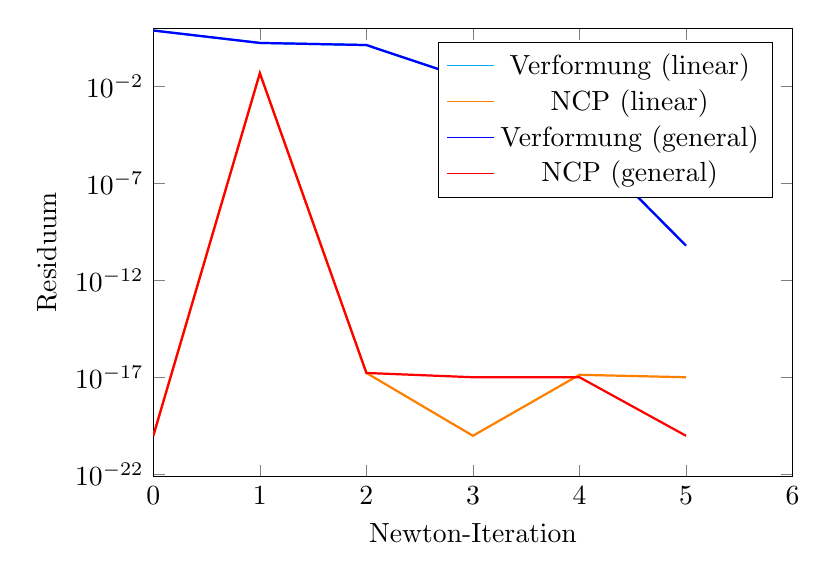
\begin{tikzpicture}[every plot/.append style={thick}] 
\begin{axis}[ 
label style={font=\normalsize}, 
xlabel={Newton-Iteration}, 
ylabel={Residuum}, 
xmin=0, xmax=6, 
ymode=log, 
ymin=0, ymax=10, 
width=0.8\textwidth, 
height=0.6\textwidth, 
legend pos=north east, 
legend style={cells={align=left}}, 
grid style=dashed, 
] 
\addplot[ 
color=cyan, 
] 
coordinates { 
(0, 7.64e+00)(1, 1.75e+00)(2, 1.36e+00)(3, 1.99e-02)(4, 2.15e-05)(5, 6.24e-11)}; 
\addlegendentry{Verformung (linear)} 
\addplot[ 
color=orange, 
] 
coordinates { 
(0, 1.00e-20)(1, 4.83e-02)(2, 1.73e-17)(3, 1.00e-20)(4, 1.39e-17)(5, 1.04e-17)}; 
\addlegendentry{NCP (linear)} 
\addplot[ 
color=blue, 
] 
coordinates { 
(0, 7.64e+00)(1, 1.75e+00)(2, 1.36e+00)(3, 1.99e-02)(4, 2.15e-05)(5, 6.24e-11)}; 
\addlegendentry{Verformung (general)} 
\addplot[ 
color=red, 
] 
coordinates { 
(0, 1.00e-20)(1, 4.83e-02)(2, 1.73e-17)(3, 1.04e-17)(4, 1.04e-17)(5, 1.00e-20)}; 
\addlegendentry{NCP (general)} 
\end{axis} 
\end{tikzpicture} 
\caption{Residuen des Stoffgesetzes 'St.Venant' mit Hinderniss 'Spitze' und 18 Freiheitsgraden für die Verschiebung.} 
\label{fiq:St.Venant_Spitze_level0} 
\end{figure} 
